\section{Proposed Taxonomy} \label{Proposed Taxonomy}

In this section we discuss our classification of speculative attacks and mitigations in Figure \ref{fig:categorization}.
This taxonomy was built from the perspective of a single core architecture.
Additionally, our threat model includes only an adversary who can arbitrarly read data from the cache and write speculative data to the cache.

For the attacks section, we separated attacks based off whether the attack is architecturally a legal action or not.
In a situation where an illegal action was performed, a fault is raised.
The different types of attacks in this section are associated with different types of faults.
However, the Page Fault has many different attacks associated with it that only differ on the permission bit abused in the attack.
This becomes another split in attack tree.
The Spectre style attacks that abuse an architecturally legal action all target different hardware modules.
This forms the split for that branch of the tree.

Defenses are organized according to implementation location and cost.
At the bottom of the stack we have the hardware mitigations, which are further divided into new modules or changed modules.
Changed modules imply a change to the function of an existing hardware component, but a new module is an entirely new hardware idea.
Firmware was seperated into it's own category because the implementation effort is drastically different than the implementation of hardware or software.
At the top, software defenses are split only into two categories, OS and application level mitigations.
This is done because both operating systems and applications cannot always be trusted.
Depending on the users threat model, a conclusion can be reached on which mitigations to assume or implement.

\begin{center}
\begin{figure}[hbtp]
    \makebox[\textwidth]{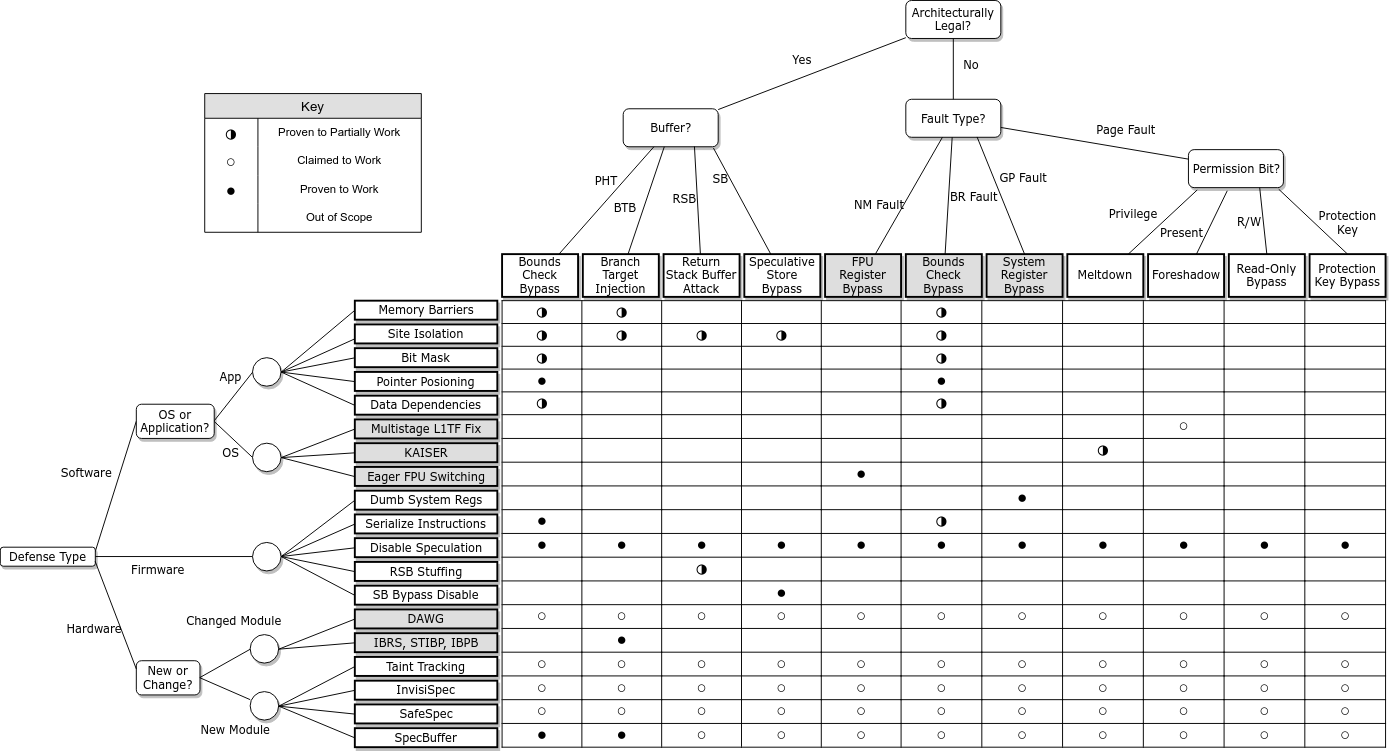
\includegraphics[width=1.1\paperwidth,angle=270]{categorization}}
    %\captionsetup{justification=centering}
	\caption{Full taxonomy of different attacks and defenses and what they cover \cite{b2, b3, b4, b8, b36, b14, b15, b16, b17, b18, b19, b20, b21, b22, b23, b24, b25, b26, b27, b28, b29, b31, b32, b33, b38, b39, b40, b41, b42, b43, b44, b45, b46}}
    \label{fig:categorization}
\end{figure}
\afterpage{\clearpage}
\end{center}
